\documentclass{standalone}
\usepackage[utf8]{inputenc}
\usepackage{tikz}
\usetikzlibrary{positioning}
\usepackage{xcolor}
\begin{document}
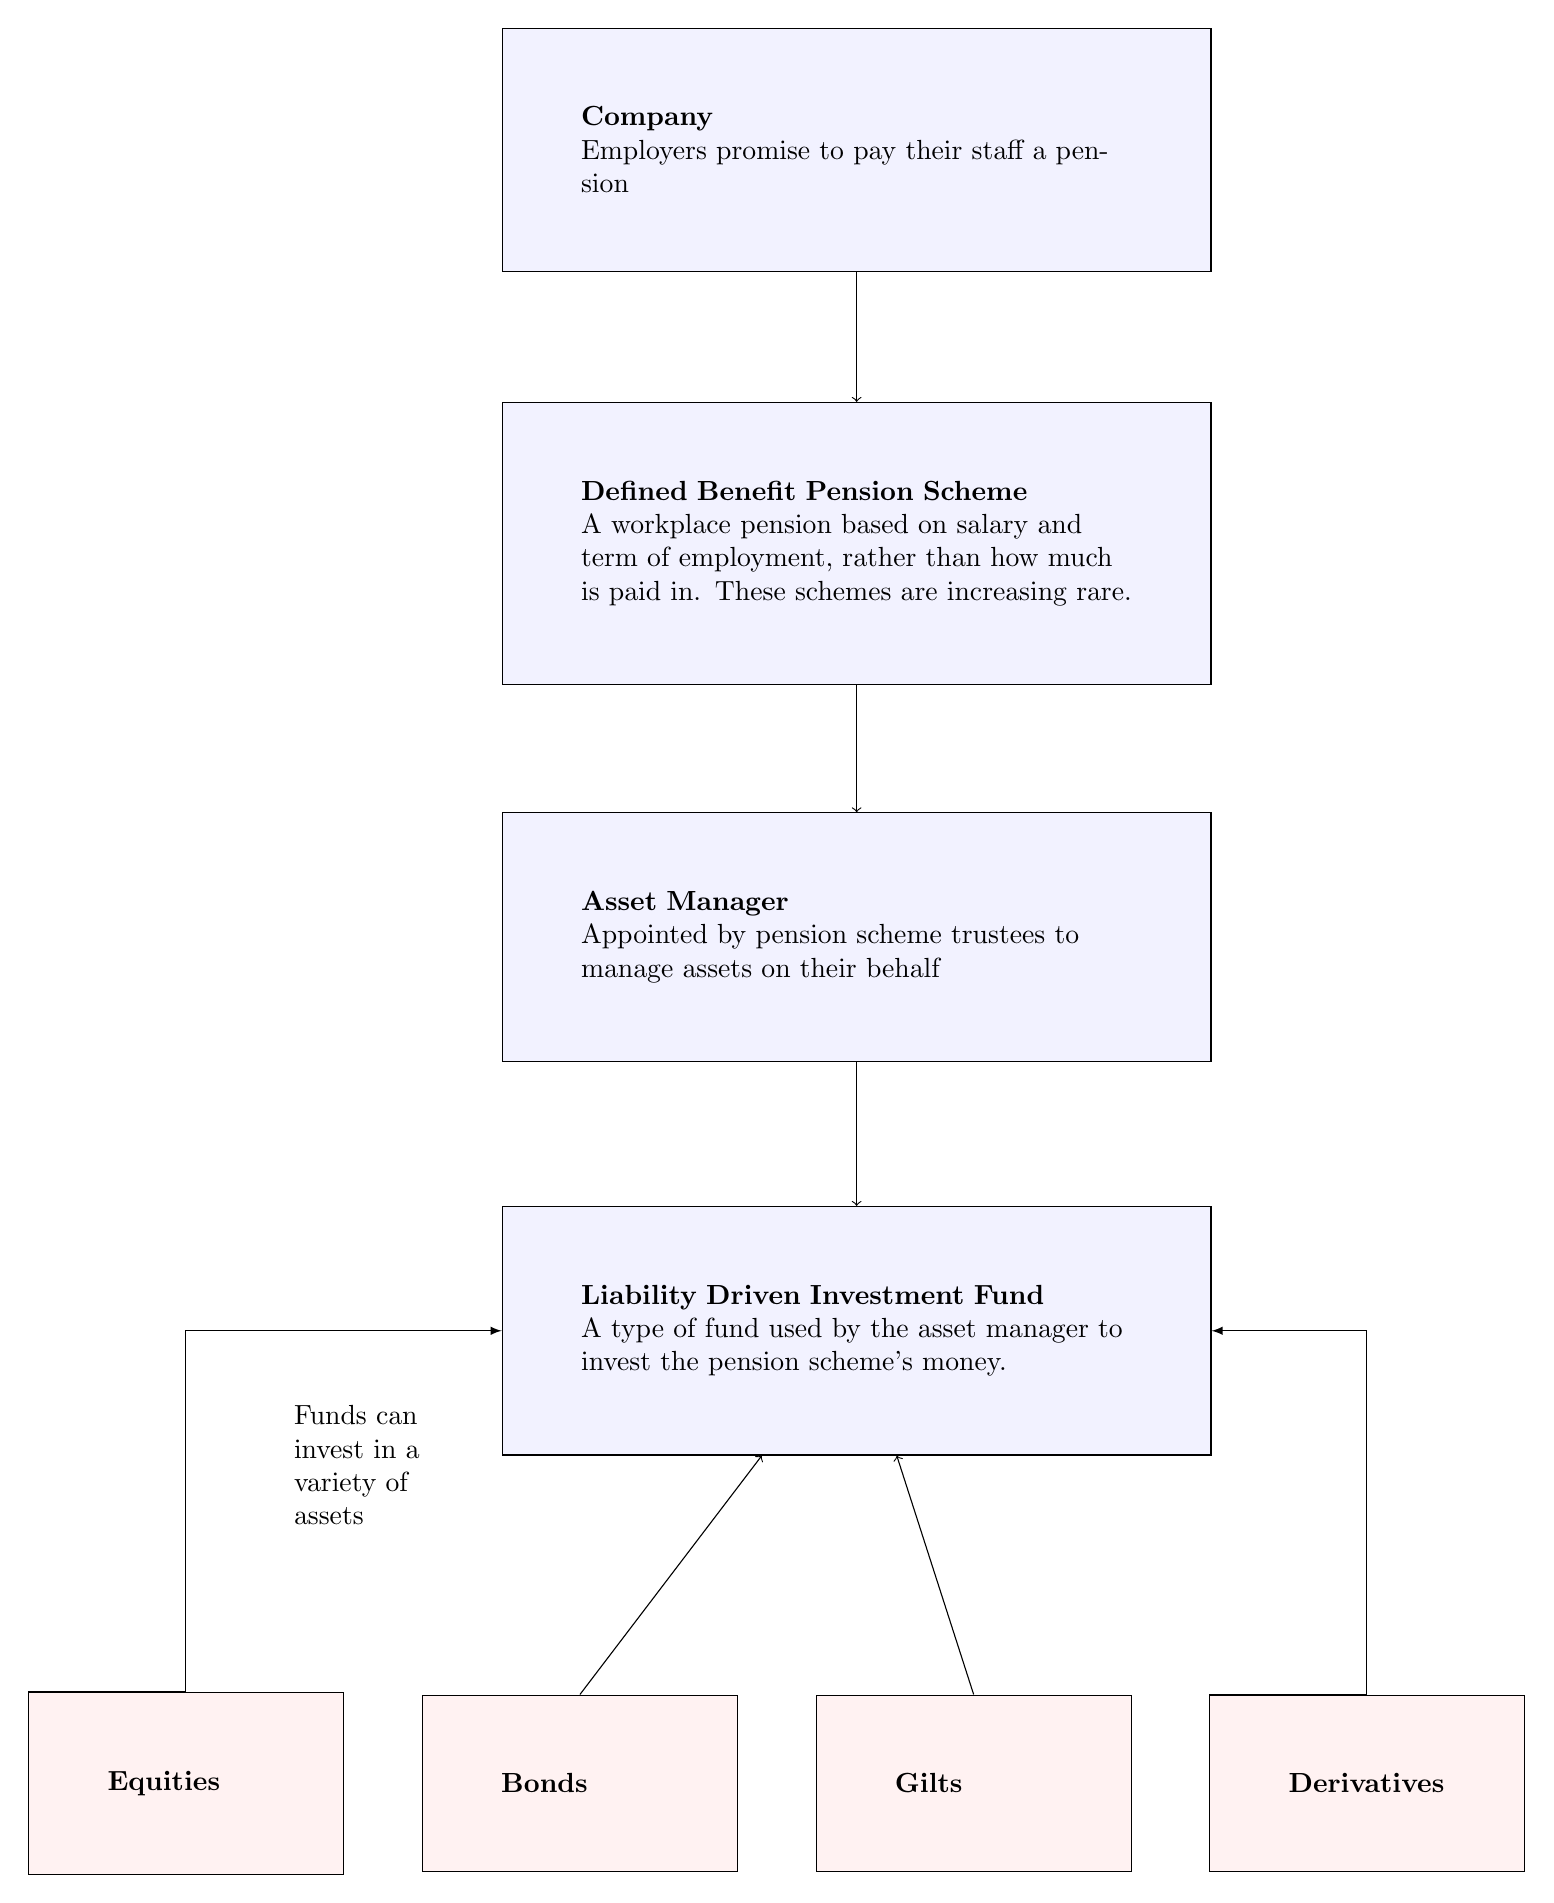
\begin{tikzpicture}[node distance=5cm]

\tikzset{
    connector/.style={
        -latex,
        font=\scriptsize
    },
    connectorReverse/.style={
        -stealth,
        font=\scriptsize
    },
    rectangle connector/.style={
        connector,
        to path={(\tikztostart) -- ++(#1,0pt) \tikztonodes |- (\tikztotarget) },
        pos=0.5
    },
    rectangle connector/.default=-2cm,
    rectangleReverse connector/.style={
        connector,
        to path={(\tikztotarget) -- ++(#1,0pt) \tikztonodes |- (\tikztostart) },
        pos=0.75
    },
    rectangleReverse  connector/.default=-2cm,
    straight connector/.style={
        connector,
        to path=--(\tikztotarget) \tikztonodes
    }
}
  \node (company) [shape=rectangle, draw, fill=blue!5, align=left, text width = 7cm,  inner sep=1cm] {
    \textbf{Company} \\
    Employers promise to pay their staff a pension
  };
  \node (pension) [shape=rectangle, draw, fill=blue!5, below of=company, text width = 7cm, align=left, inner sep=1cm] {
  \textbf{Defined Benefit Pension Scheme} \\
    A workplace pension based  on salary and term of employment, rather than how much is paid in. These schemes are increasing rare.
  };
  \node (asset) [shape=rectangle, draw, fill=blue!5, below of=pension,  text width = 7cm, align=left, inner sep=1cm] { \textbf{Asset Manager} \\
  Appointed by pension scheme trustees to manage assets on their behalf} ;
  \node (fund) [shape=rectangle, draw, fill=blue!5, below of=asset,  text width = 7cm, align=left, inner sep=1cm] { \textbf{Liability Driven Investment Fund} \\ 
  A type of fund used by the asset manager to invest the pension scheme's money.
  };
  \draw [->] (company) -- (pension);
  \draw [->] (pension) -- (asset);
  \draw [->] (asset) -- (fund);


   \node (equities) [shape=rectangle, draw, fill=red!5, below left=3cm and 2cm of fund, text width = 2cm, align=left, inner sep=1cm] { \textbf{Equities}};
  \node (bonds) [shape=rectangle, draw, fill=red!5, right of=equities, text width = 2cm, align=left, inner sep=1cm] { \textbf{Bonds}};
  \node (gilts) [shape=rectangle, draw, fill=red!5, right of=bonds, text width = 2cm, align=left, inner sep=1cm] { \textbf{Gilts}};
  \node (derivatives) [shape=rectangle, draw, fill=red!5, below, right of=gilts, text width = 2cm, align=left, inner sep=1cm] { \textbf{Derivatives}};

  \node [above left=2cm and -5.5cm of equities, align=left, text width=2cm] {Funds can invest in a variety of assets};
  \node (fwaypoint)[draw=none, below =1.75cm of fund] {};
  % \draw [-] (fund.south) to (fwaypoint);
  \draw [-stealth, rectangleReverse connector=2cm] (fund.west) to (equities.north west);
  \draw [-stealth, rectangleReverse connector=2cm] (fund.east) to (derivatives.north west);
  \draw [->] (bonds.north) to (fund);
   \draw [->] (gilts.north) to (fund);
\end{tikzpicture}

\end{document}
